\section{Design of \arch}
{\bf Kartik's Note: This section is a placeholder. Contents moved to respective hypervisor/container sections.}

In this section, we introduce the design of \arch. 
The key idea is that instead of copying VM/container memory while replacing a hypervisor/OS, \arch relocates the memory ownership of VMs/containers from the stale hypervisor/OS to the replacement hypervisor/OS using a new data structure, \arch table. The per-VM (or per-process) \arch table stores the memory mappings from the pages of a VM (or a container) to the  pages of the physical memory, constructed by the current (to-be-stale) hypervisor/OS, and is leveraged by the new hypervisor for reconstructing the memory address space of the VM (and the process) during hyerpervisor/OS replacement. Such memory ownership relocation is fast and leads to a live hypervisor/OS replacement. In addition, \arch brings a bunch of optimizations to further mitigate possible overhead especially the overhead brought by nested virtualization.

%The key design goals of the proposed work are transparency and minimum 
%service disruption in guests. The architecture of live hypervisor replacement
%is shown in Figure~\ref{fig:arch}. Using nested virtualization, the hypervisors at L1 and unmodified guests are run on thin hyperplexor at L0. Using SR-IOV, a single PCI device or physical function is presented as multiple virtual functions to hypervisors to reduce the performance overhead in guest due to nested virtualization. Upon a migration event, an updated hypervisor is first started on thin hyperplexor. The updated hypervisor then replaces the aged hypervisor by co-mapping the memory of guest. The hyperplexor transfers the memory mappings using grant table mechanism where the  guest page frames are mapped to the updated hypervisor followed by unmapping of memory from the aged hypervisor. The completion of hypervisor replacement is marked by pausing the guest and transferring the vCPU and I/O states to the updated hypervisor.  

%In the remaining section, we describe 1. How the memory mappings of guest are transferred between hypervisors using grant table mechanism 2. How we reduce the performance overhead due to nested virtualization.  
\begin{figure}[t!]
 	  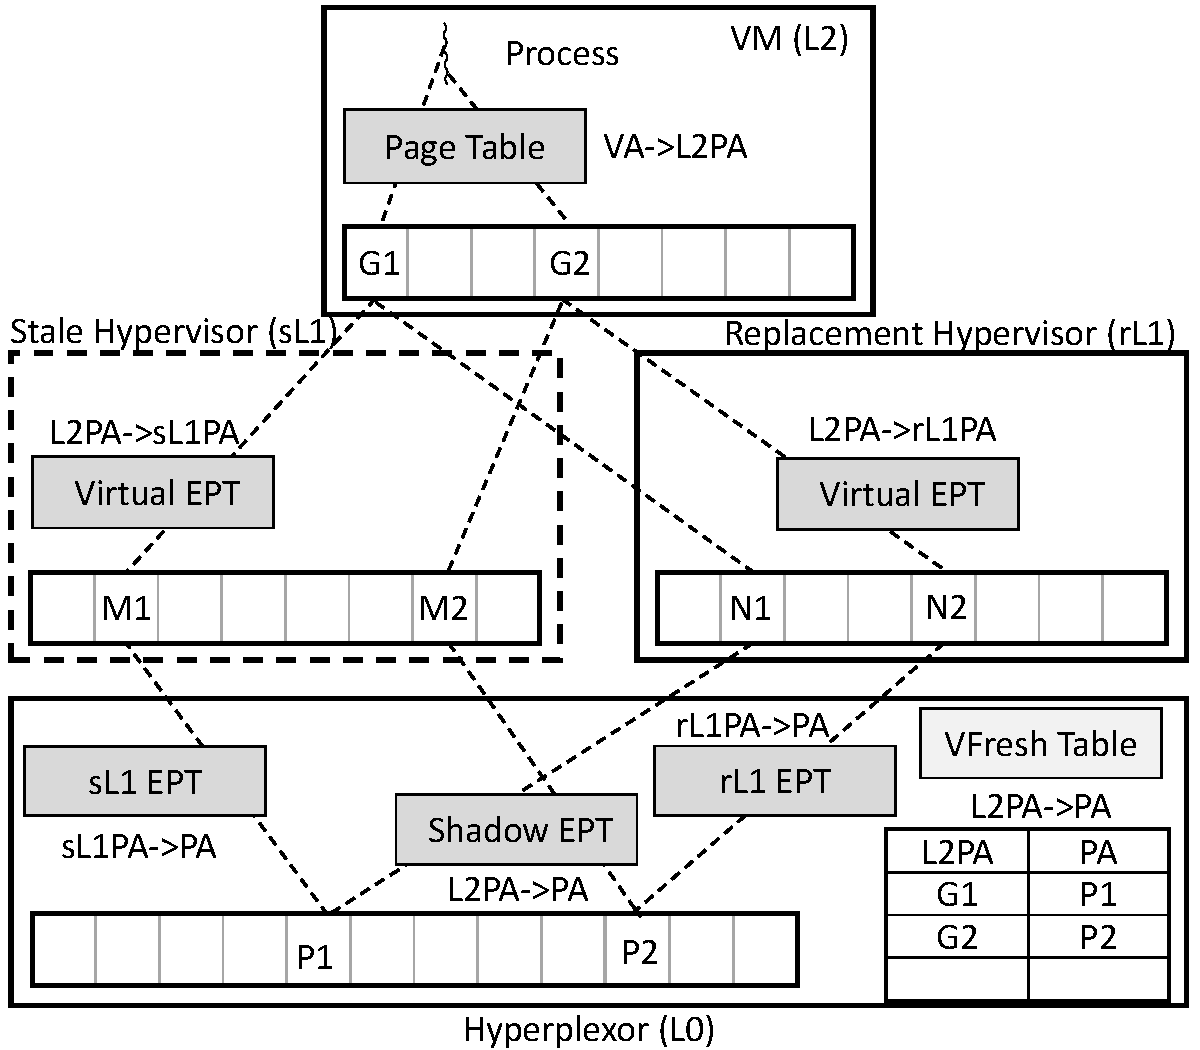
\includegraphics[width=0.45\textwidth]{figures/vfresh-table.pdf}
  \caption{Memory management for nested virtualization.}
  \label{fig:mapping}
  %\includegraphics[width=15cm,height=6cm,keepaspectratio]{architecture__1_.jpg}
\end{figure}

\subsection{Hypervisor Replacement}
We first introduce memory management under nested virtualization, followed by the design of the \arch table and the hypervisor switching based on the \arch table, and finally the optimizations to mitigate the overhead of nested virtualization.

\subsubsection{Memory Management}
In native (without virtualization), a page table stores the mappings between the virtual addresses (VA) of a process to its physical addresses (PA) where data content actually resides. With such mappings, once VAs are accessed by the process the hardware memory management unit (MMU) can do VA-to-PA translations automatically. 

In single-level virtualization, an additional level of memory address translation (in hypervisor) is added for virtualizing memory management of VMs and providing isolation between VMs. In consequence, the page table of a process running on a VM stores the mappings between the guest virtual addresses (GVA) of a process and the guest physical addresses (GPA). The hypervisor uses a hardware-assistant page table EPT to map guest physical addresses to host physical addresses (GPA to PA). Initially, the EPT of the VM is empty. When the VM tries to access its physical addresses, VM page faults, or EPT violations, are generated, like page faults for a process. These faults are processed by the hypervisor which allocates pages for the faulting GPA. 

As illustrated in \fref{fig:mapping}, in nested virtualization, three levels of translations are needed. A process's virtual address is translated to GPA, or physical address of L2 VM (L2PA). An L2PA is translated to the physical address of the L1 hypervisor (L1PA) using a virtual EPT for the associated VM maintained by the L1 hypervisor. Finally, L1PA is translated to the physical address of the host (PA) using the EPT for the L1 hypervisor maintained by the hyperplexor at L0. Since, the MMU can translate only two levels of memory mappings, the hyperplexor at L0 combines the virtual EPT at L1 hypervisor and the EPT at L0 to construct a shadow EPT for every L2 VM, used for translating L2PA to PA. The shadow EPT is updated as the updates of the virtual EPT at L1 and/or EPT at L0 take place via the EPT violations mechanism. Thus, the MMU uses the process page table in the L2 VM and the shadow EPT at L0 to translate a process virtual address to the PA.
 
 \begin{table*}[!htb]
\small
  \begin{tabular}{|c|l|l|l|}
   \hline
  \arch API & \multicolumn{1}{c|}{Input Parameters} & \multicolumn{1}{c|}{Return Value} & \multicolumn{1}{c|}{Description}\\
  \hline
  \hline
  hypercall\_set &unsigned long base\_addr\_of\_l2gfn\_list, &0 on success,  & Given the VM on the stale hypervisor, \\ 
  &unsigned long base\_addr\_of\_l1gfn\_list, &failure code otherwise & pass a list of L2-to-L1 page mappings to hyperplexor  \\
  &unsigned int count, & & for setting up \arch table entries  \\
  &unsigned int vmid & & storing the L2-to-PA page mappings\\
  \hline

  hypercall\_map &unsigned long base\_addr\_of\_l2gfn\_list, &0 on success, & Given the VM on the replacement hypervisor, \\
  &unsigned long base\_addr\_of\_l1gfn\_list, &failure code otherwise & pass a list of L2-to-L1 page mappings to hyperplexor \\
  &unsigned int count, & & to look up \arch table  \\
  &unsigned int vmid && for creating L2-to-PA mappings\\
  \hline
  
    hypercall\_set &unsigned long base\_addr\_of\_gva\_list, &0 on success,  & Given a process on the stale OS, \\ 
  &unsigned long base\_addr\_of\_gfn\_list, &failure code otherwise & pass a list of process-to-VM page mappings   \\
  &unsigned int count, & & to hypervisor for setting up \arch table entries  \\
  &unsigned int pid & & storing the GVA-to-PA page mappings\\
  \hline

  hypercall\_map &unsigned long base\_addr\_of\_gva\_list, &0 on success, & Given the process on the replacement hypervisor, \\
  &unsigned long base\_addr\_of\_gfn\_list, &failure code otherwise & pass a list of process-to-VM page mappings\\
  &unsigned int count, & & to look up \arch table  \\
  &unsigned int pid && to hypervisor for creating GVA-to-PA page mappings\\
  \hline
\end{tabular}
\caption{\arch API}
\vspace{-0.2in}
\label{tab:api}
\end{table*}

\subsubsection{\arch Table}
Instead of copying a VM's memory while replacing its hypervisor, \arch relocates the memory ownership of the VM from the stale hypervisor to the replacement hypervisor. To achieve this, \arch builds a new page table, {\em \arch table}, in the hyperplexor at L0. The \arch table stores the page mappings of L2-to-PA for the VM by the stale hypervisor, and is used for reconstructing the same L2-to-PA page mappings for the VM on the replacement hypervisor.

To establish the \arch table, the hyperplexor needs a list of L2-to-L1 page mappings of the VM from the stable hypervisor (i.e., using the virtual EPT table). \arch provides a hypercall, \texttt{hypercall\_set}, to the stale hypervisor for exposing such mappings, as listed in Table \ref{tab:api}. The stale hypervisor invokes this hypercall to pass a list of L2-to-L1 page mappings of the VM to the hyperplexor. For each received L2-to-L1 page mapping, the hyperplexor translates the L1 page number to the PA page number (i.e., using the EPT table at L0), and puts the corresponding L2-to-PA page mapping to the {\em \arch table} (associated with the VM's ID). The stale hypervisor can invoke multiple \texttt{hypercall\_put} hypercalls to pass all necessary L2-to-L1 page mappings for fully setting up the \arch table for the VM.

Relocating memory ownership of the VM on the replacement hypervisor needs to map its L2 pages (newly allocated) to the same physical pages as the VM on the stale hypervisor, using the \arch table. To establish such mappings, the hyperplexor again needs a list of L2-to-L1 page mappings of the VM from the replacement hypervisor via a new hypercall, \texttt{hypercall\_map}. We will shortly see how the L2-to-L1 mappings are constructed on the replacement hypervisor. The replacement hypervisor invokes this hypercall to pass a list of L2-to-L1 page mappings of the VM to the hyperplexor. For each received L2-to-L1 page mapping, the hyperplexor: (1) looks up the {\em \arch table} to find the L2-to-PA mapping with the L2 page number as the key; and (2) installs the L1-to-PA page mapping in the replacement hypervisor's EPT table \footnote{In fact, \arch translates the GVA to host physical address (HVA) of the VM (maintained by kvm), install the HVA-to-PA page mapping in the page table of the VM's QEMU process, and last invalidates the entry of the EPT table, which will be updated later.}. Similarly, the replacement hypervisor can invoke multiple \texttt{hypercall\_map} hypercalls to pass all L2-to-L1 page mappings for fully relocating memory ownership of the VM from the stale hypervisor to the replacement hypervisor. 
%In our approach, we leverage grant table mechanism to transfer the mappings of guest from current hypervisor to updated hypervisor. The current hypervisor requests the hyperplexor to create grant entries in grant table. The updated hypervisor then requests the hyperplexor to map the guest page frame to physical page frames. 

%\textbf{\textit{Background}}
%In Xen, Virtual Machine Monitor (VMM) runs at the highest privilege level which coordinates with host domain (Dom0) or host OS to maintain isolation between guest domains (DomU) or guest OS. Xen supports both full-virtualization and para-virtualization modes. Para-virtualization mode is more efficient with lower virtualization overhead. However, it comes with a trade-off of modifying the guest OS.

%In Xen, the devices are managed by native device drivers run in isolated driver domain (IDD). The network device is presented as a virtual network device to a guest OS. The guest OS runs the front-end driver which shares a device ring buffer with the back-end driver in IDD or Dom0. In para-virtualization mode, a grant table\cite{Pratt05xen3.0} is used as a communication channel between domains. Each domain has a grant table and it is used to share or transfer the memory mappings between the domains. A grant table data structure is shared between Xen and the domain. The grant table entries are indexed using an integer field called grant reference. The reference field indicates which grantee can share the pages with the granter. 

%To share the pages, the granting domain advertises the page to be shared with other domains. The granting domain shares the grant reference ID with the receiving domain. The receiving domain maps the page by updating it's grant table entry. After the receiving domain has finished the operation on the page, the granting domain revokes the access to the page. For page transfer mechanism, after the granting domain transfers the page to the receiving domain, the page is freed from the granting domain. Transferring the pages between the domains reduces the memory-copy overhead which increases with increase in data-size.   



\subsubsection{Hypervisor Switching}
%In the proposed work, we use grant table to share and finally transfer the ownership of the physical page frames from old hypervisor to the current hypervisor. As shown in Figure~\ref{fig:mapping}, the grant table is maintained by the hyperplexor which is responsible to transfer the ownership of the guest memory. The grant table holds the list of all the guest page frame mappings to the memory page frames. It also contains a guest ID field which signifies the ownership of the guest page frames.

A VM, e.g., VM1, initially runs on the hypervisor (L1) which in turn runs on the thin hyperplexor (L0). During boot time, VM1 pre-allocates its memory by pinning the L2 pages in memory (i.e., the swap option is disabled). By doing this, the virtual EPT for VM1 in its L1 hypervisor and the shadow EPT in the L0 hyperplexor get populated, resulting in no further virtual EPT or shadow EPT faults during the runtime. The \arch table is created when VM1 requests the L1 hypervisor to pin all the L2 pages --- the L1 hypervisor invokes a series of \texttt{hypercall\_set} hypercalls each with a list of L2-to-L1 page mappings (i.e., from the virtual EPT), and the hyperplexor uses received mappings to populate the \arch table for VM1 as stated above.

%and for the guest in the hyperplexor during the boot time.  As the guest memory pages are pinned in memory and the swap option is turned off the memory mappings of the guest are not bound to change.


When VM1's current hypervisor needs updates, a replacement hypervisor (with pre-installed updates) boots up (co-existent with the stale hypervisor). The replacement hypervisor prepares a new VM, VM2, in the {\em replacement} state (i.e., not running). VM2 is allocated with the same range of L2 pages as VM1, and then requests the replacement hypervisor to map its L2 pages to the same physical pages as VM1. The replacement hypervisor first gets the free L1 pages to map the L2 pages in VM2's virtual EPT. Note that, such L1 pages are not necessary to be the same as that in VM1's hypervisor as shown in \fref{fig:mapping}. After populating the L2-to-L1 page mappings, the replacement hypervisor invokes a series of \texttt{hypercall\_map} hypercalls each with a list of L2-to-L1 page mappings to the hyperplexor. The hyperplexor installs the L1-to-PA page mappings in the replacement hypervisor's EPT table using the \arch table, as stated above. 

At this stage, VM2 still stays in the replacement state (i.e., not running) and hence does not corrupt the memory of VM1. VM2 waits for the VCPU and I/O device state of VM1 before starting running. VM1 on the stale hypervisor is then paused and the VCPU and I/O device state are transferred to VM2 on the replacement hypervisor.  Once VM1 is paused, the VM ID of the \arch table is changed to the VM2's ID. 

Finally, once the control of VM1 is transferred to the replacement hypervisor, the stale hypervisor can safely unmap VM1's memory from its address space and be safely powered off. With all the state of VM1, the replacement hypervisor starts VM2, which resumes the running state from where VM1 is paused.  The replacement hypervisor becomes the current hypervisor. 


%As shown in Figure~\ref{fig:mapping} when the updated hypervisor has to replace the current hypervisor, the guest QEMU that runs on updated hypervisor before the migration requests updated hypervisor to map it's guest page frames to the physical page frames in advance using the grant table. The hyperplexor maps the new guest page frames to physical page frames using grant table. At this stage, the QEMU on updated hypervisor is in migrate state and does not corrupt the memory as it does not contain the current vCPUs and I/O device information. This maintains the consistency in memory. As a result the ownership of the physical page frames in grant table is not yet transferred to the new guest.    

 

\begin{figure}[t!]
  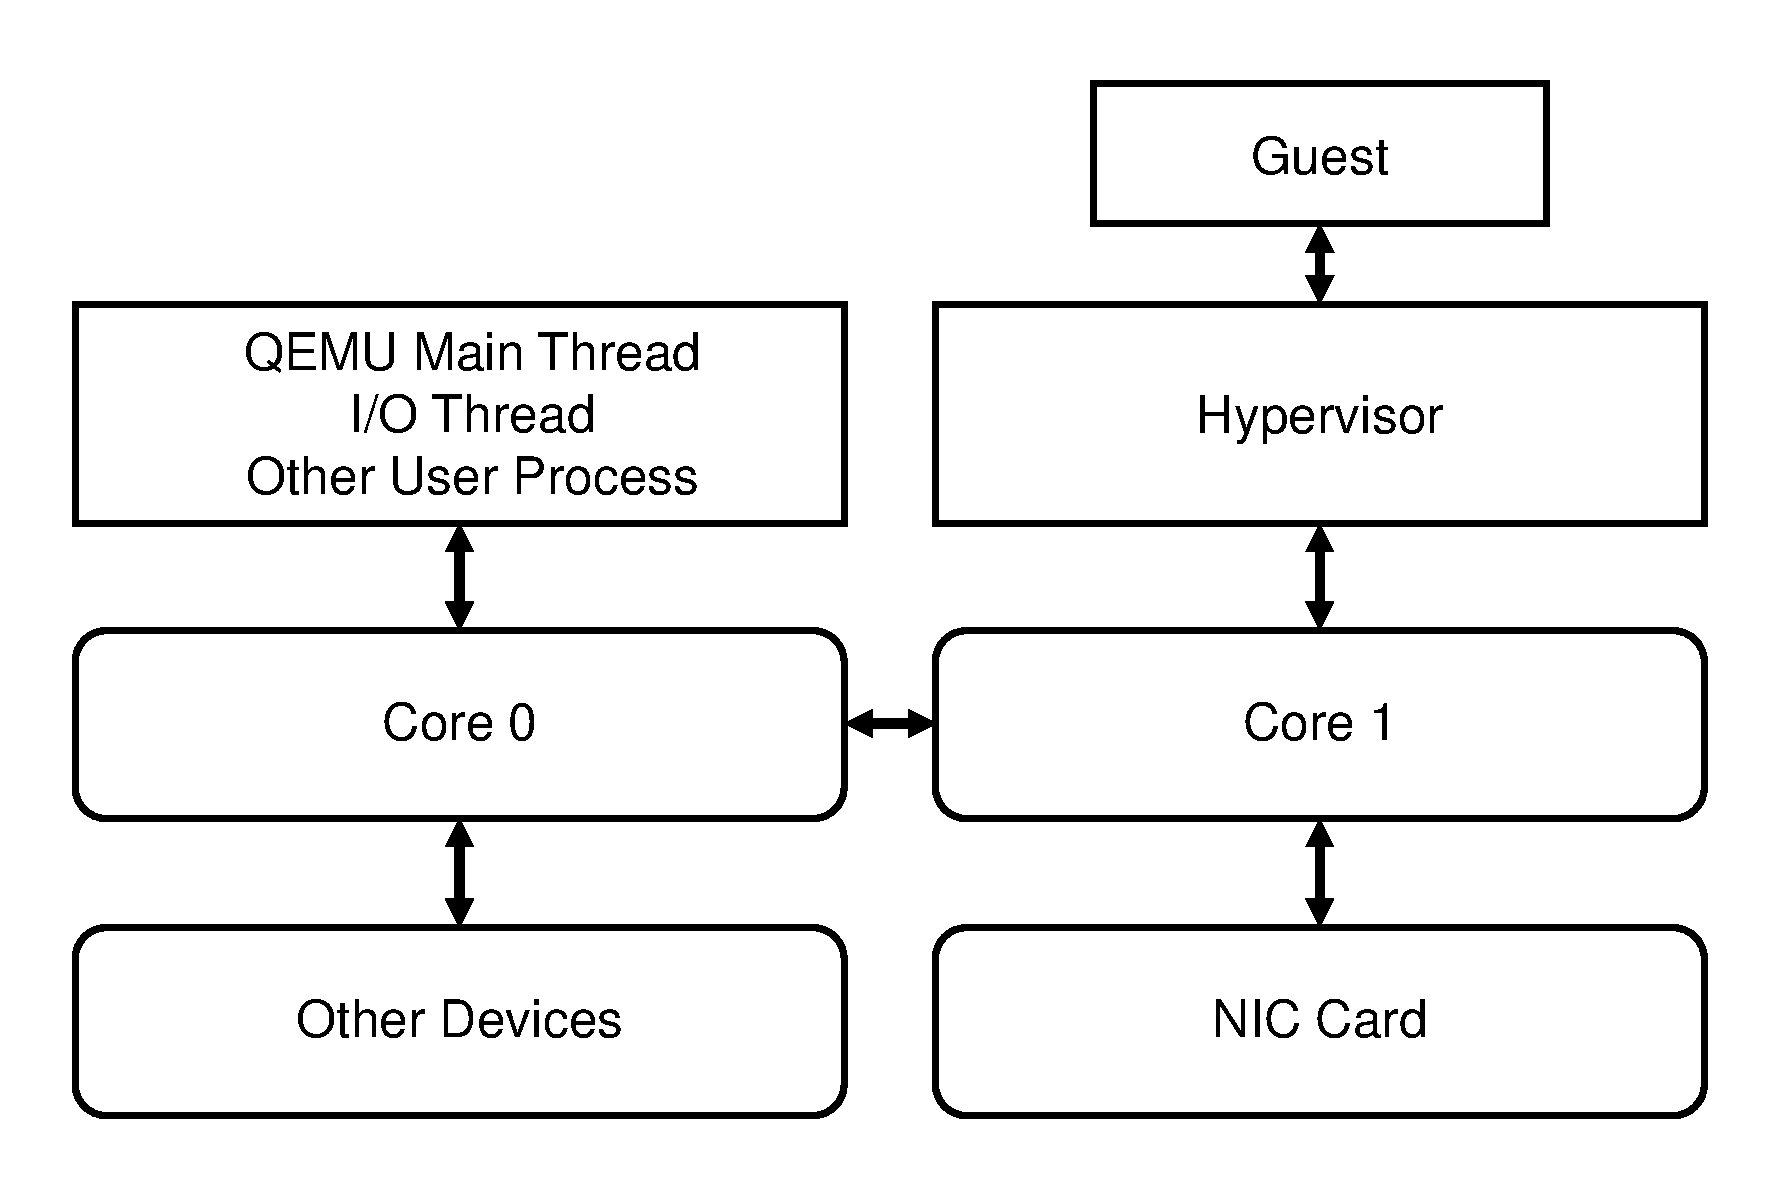
\includegraphics[width=0.4\textwidth]{figures/nested_virtualization_overhead_setup.pdf}
  \caption{Optimizations to reduce overhead of nested virtualization}
  \label{fig:optimizations}
  %\includegraphics[width=15cm,height=6cm,keepaspectratio]{architecture__1_.jpg}
\end{figure}

\subsubsection{Nested Overhead Mitigation}
In comparison with the traditional single-level virtualization 
setup, where the hypervisor directly controls the hardware,
nested virtualization can introduce additional emulation overheads, especially for I/O virtualization. To mitigate such overhead, \arch uses the direct device assignment of network interface cards (NIC) to the hypervisor. 

%\textbf{Background}
Existing virtualization techniques (e.g., KVM \cite{kivity2007kvm}) support the full virtualization mode through device emulation \cite{sugerman2001virtualizing} and para-virtualization using virtio drivers \cite{russell2008virtio, barham2003xen}  in VMs. 
%They also support direct device assignment  to the guest \cite{ben2006utilizing}. 
For example, QEMU \cite{bellard2005qemu} emulates I/O devices requiring no modifications to VMs. When VMs access the devices, the I/O instructions are trapped into hypervisor leading to a number of VM/host context switches, resulting in lower performance of VMs. The para-virtualized devices offer better performance compared to device emulation, as the modified drivers in VMs avoid excessive VM/host switches for the I/O workloads. With Intel's VT-d \cite{abramson2006intel}, direct device assignment offers improved performance, as VMs directly interact with the devices bypassing the hypervisor.    
%With hardware virtualization technology, 
Further, SR-IOV \cite{dong2008sr} enables a single network device to present itself as multiple virtual NICs to VMs through virtual functions (VFs). Using a VF, a VM directly interacts with the network device --- with Intel's hardware support, VMs can directly access device memory through IOMMU which converts VMs physical addresses to host physical addresses.

%\textbf{Direct Device Assignment of Network Interface Card}
In this paper, \arch uses VFs to achieve network performance in nested guest to match the performance of a single-level guest and minimize the CPU Utilization in hyperplexor. VFIO \cite{vfiodriver} driver supports direct device assginment to a virtual machine. As shown in \fref{fig:vFresharch}. every hypervisor running on hyperplexor is assigned one virtual function. The guest running on hypervisor uses para-virtualized driver to run the I/O workloads. \arch further applies many optimizations to provide hypervisor with enough resources and reduce the CPU utilization on hyperplexor. The goal is to run the hypervisor with minimum hyperplexor intervention. We describe the optimization techniques in detail in the following sections.

\begin{figure}[t!]
 	  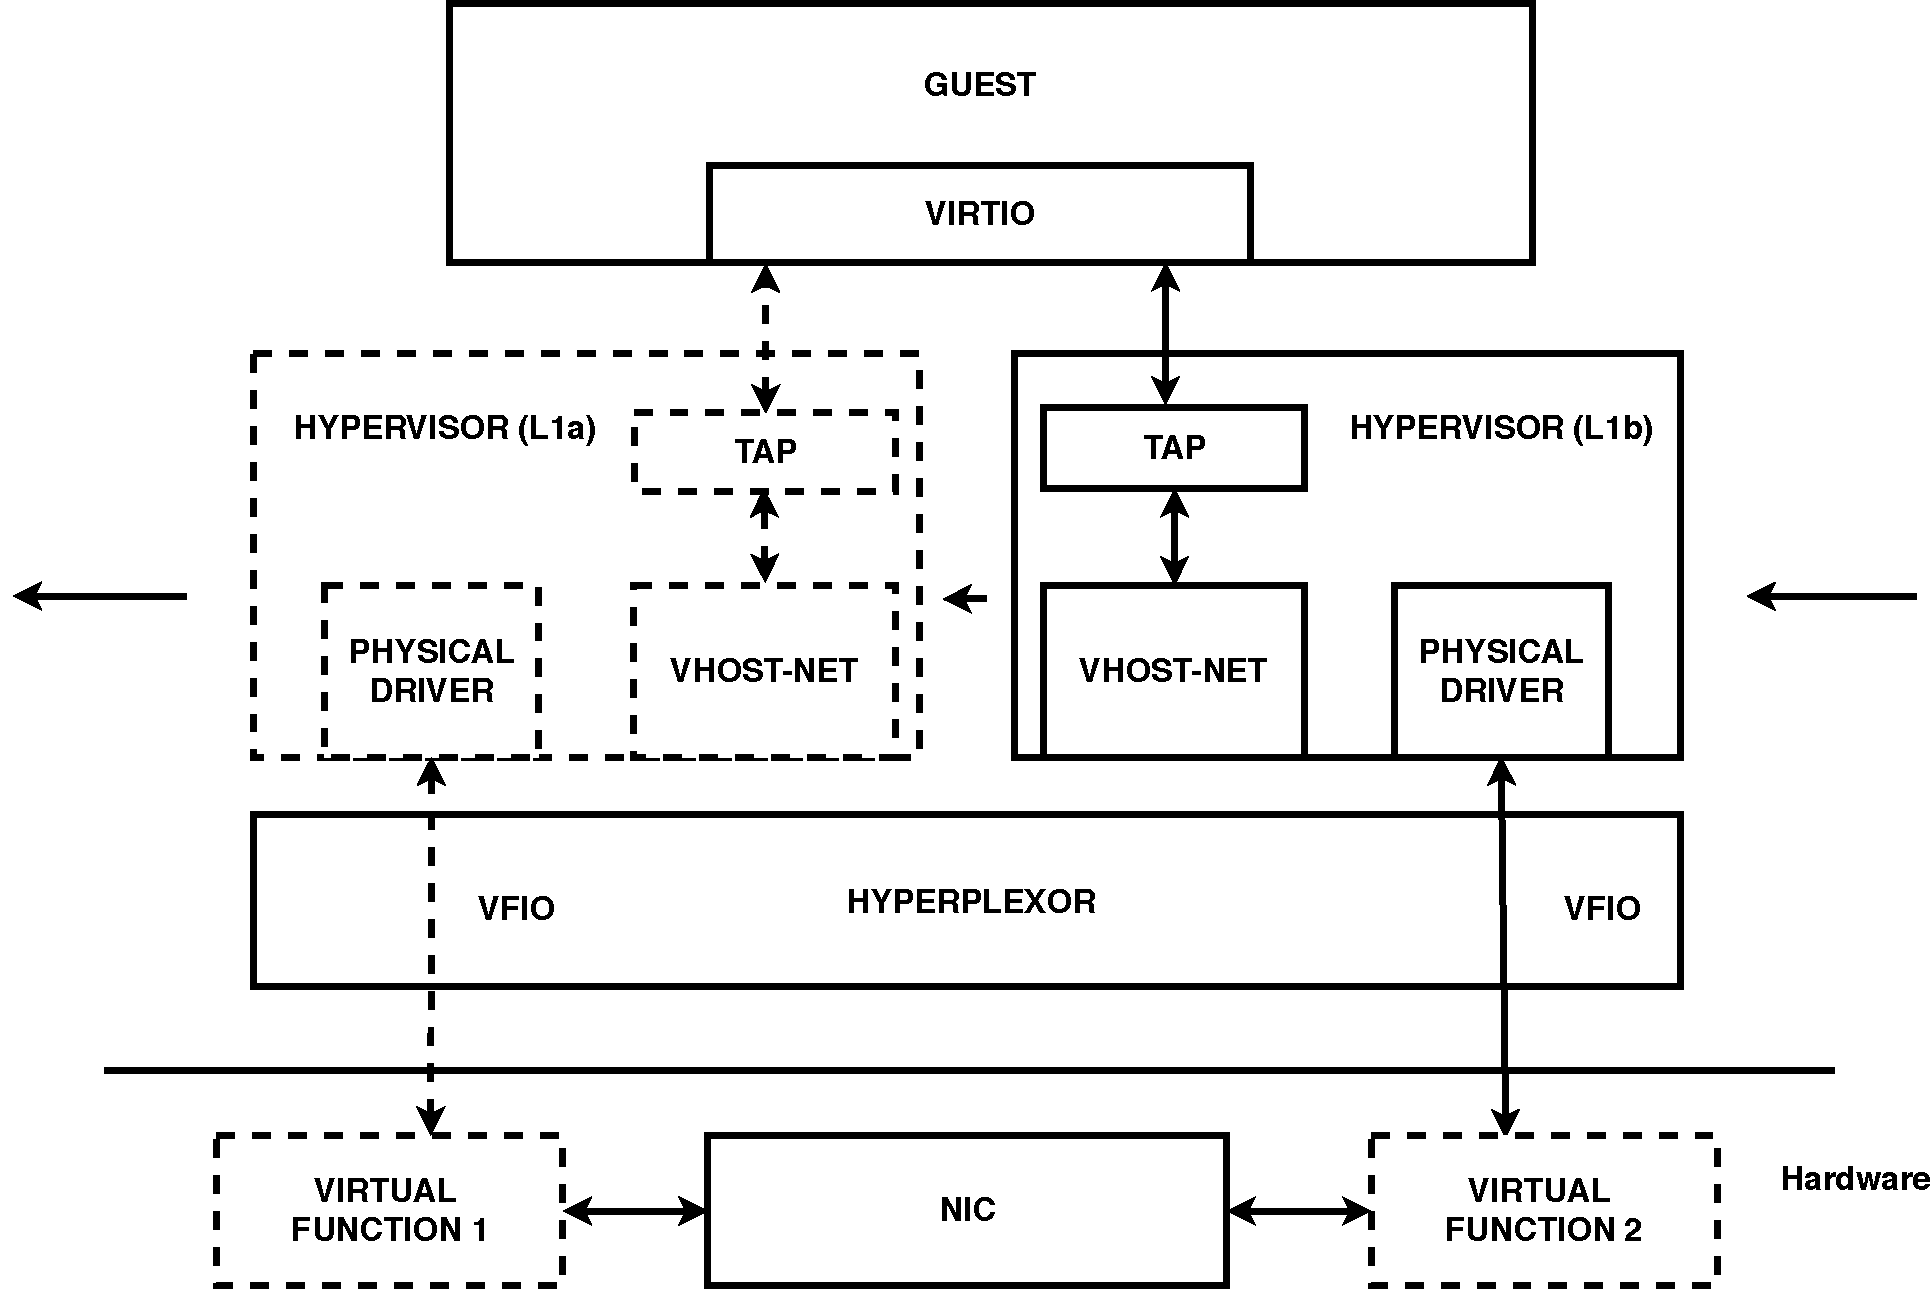
\includegraphics[width=0.45\textwidth]{figures/architecture_modified.pdf}
  \caption{Memory management for containers.}
  \label{fig:vFresharch}
  %\includegraphics[width=15cm,height=6cm,keepaspectratio]{architecture__1_.jpg}
\end{figure}

%\begin{itemize}
%\item \textbf{\textit{Reducing Memory Footprint of Hyperplexor}}
\para{Memory Footprint.}
As the hyperplexor involvement is minimal, it is configured with essential packages, device drivers and services reducing the memory consumption. The size of the hyperplexor without VM is 90 MB of the available memory compared to the Ubuntu server size 154 MB. The userspace processes and services that where not necessary to run the L1 hypervisor with direct-device assignment were identified and removed. The Linux kernel 4.13 is compiled with 32 kernel modules compared to 120 kernel modules in Ubuntu server. 
    
%	\item \textbf{\textit{HLT Exits}}
%halt_poll_ns is a kvm kernel module parameter. When guest VCPU has no work to do or goes idle, the VCPU goes to sleep by executing HLT instruction which causes a VM Exit. The parameter halt_poll_ns specifies how much time the VCPU needs to poll before executing the HLT instructions. This polling interval helps in making the guest more responsive for workloads like the network.

\para{HLT Exits.}
Although a directly assigned network device to a VM gives better performance, the CPU utilization on the host is high due to the idle polling of VCPUs. When the VM is idle, QEMU halts the idle VCPUs by executing a HLT instruction which triggers a VM exit. When the work is available for the VCPU, it has to be woken up to execute the new work. This transition from idle to ready state is costly as it involves context switch and hinders the performance of the VM. To avoid too many transitions, before executing the HLT instruction the VCPU polls for the specified amount of time to check if there is any additional work to be executed. This idle polling of VCPUs reduces the number of VM exits but increases CPU utilization on host. To reduce CPU utilization on host, we disable polling of VCPUs before executing HLT instruction. 
KVM provides a halt\_poll\_ns kernel module parameter to set the value of halt\_poll\_ns. To disable polling we set halt\_poll\_ns to zero. In this paper, as we assign the network device to the hypervisor, we disable the halt polling on the hypervisor to reduce the CPU Utilization in host.
    
   %\item \textbf{\textit{Posted Interrupts}}
\para{Posted Interrupts.}
     When an external interrupt arrives, the CPU switches from non-root mode to root mode (VM Exit) and transfers the control to the hypervisor. Increase in number of external interrupts causes increase in VM Exits. With Intel's VT-d posted interrupt support the external interrupts are delivered to guest without hypervisor intervention. With posted interrupts support the hypervisor can inject a virtual interrupt to guest by updating the fields in the VMCS in guest or non-root mode. Hypervisor notifies the arrival of posted interrupt to the guest by setting the fields Posted Interrupt Request (PIR), Notification Vector (NV) and Outstanding Notification (ON) in Posted Interrupt Descriptor structure. The PIR field is 256 bit long and provides storage for posting the interrupts. The NV field is used to notify the interrupt vector to the guest. The ON bit indicates the processing status of the posted interrupt. We enable posted interrupt feature on the hyperplexor and deliver external interrupts directly to hypervisor without causing exits to hyperplexor.  
     
%\item \textbf{\textit{Dedicated Cores}}
\para{Dedicated Cores.}
All the system processes are run on two cores except the VCPUs which run on dedicated cores. The VCPUs are assigned dedicated cores to eliminate other processes from contending with VCPUs. As shown in Figure~\ref{fig:optimizations}. the QEMU process along with other hyperplexor processes are pinned to CPU0 and the hypervisor VCPUs run on the dedicated cores. 

\begin{figure}[t!]
 	  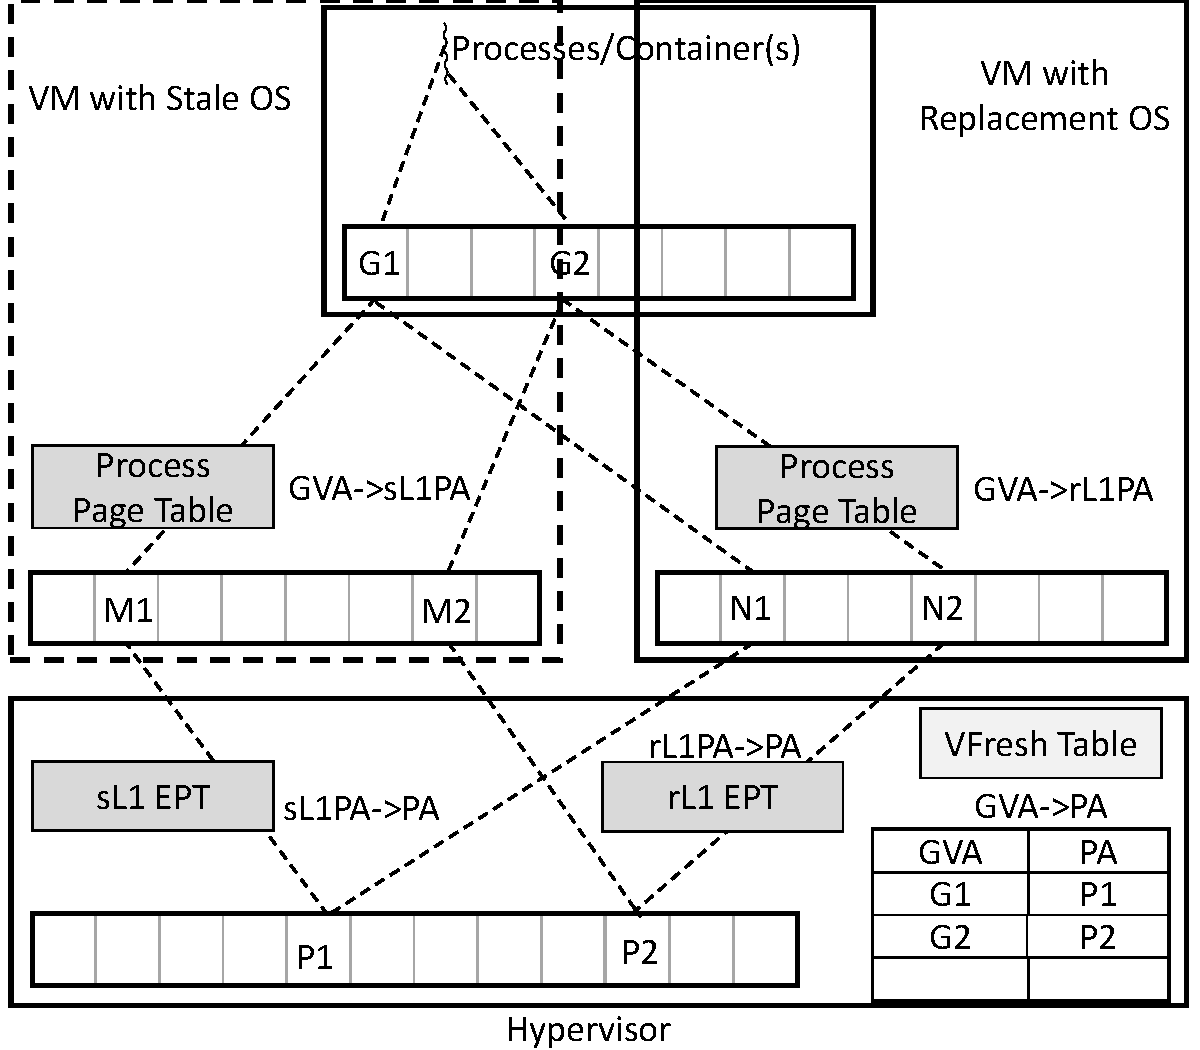
\includegraphics[width=0.45\textwidth]{figures/vfresh-table-container.pdf}
  \caption{Memory management for containers.}
  \label{fig:mappingc}
  %\includegraphics[width=15cm,height=6cm,keepaspectratio]{architecture__1_.jpg}
\end{figure}

\subsection{OS Replacement}
Using containers to host applications becomes a common usage scenario in today's cloud~\cite{aws, gcpkubernetes, azureks, ibmkubernetes, vmwarepks}. Under this scenario, the process of OS replacement can be viewed as moving the state of all containers from the old VM with the stale OS to a new VM with the replacement OS. Again, we leverage intra-host live migration to avoid inter-host communication.

Essentially, a container consists of a hierarchy of processes as well as isolation mechanisms (e.g., \texttt{cgroups} and \texttt{namespaces} in Linux). If not specified, processes running upon an OS belong to a default container. Hence, moving a container from one VM to another for OS replacement needs to copy the state of all processes in the container from one VM to another. Again, \arch's OS replacement relocates the memory ownership of all processes instead of copying memory data. The design of \arch's OS replacement is  similar to the above hypervisor replacement, and we focus on the differences in the OS replacement.

\subsubsection{Memory Management}
The memory management under the container case belongs to the above-mentioned single-level virtualization. As shown in \fref{fig:mappingc}, the page table of a process (in a container) running in the VM stores the mappings between the guest virtual addresses (GVA) of the process and the guest physical addresses (GPA) of the VM. The hypervisor uses the EPT to map GPA to physical addresses (PA). 

\subsubsection{\arch Table}
To build the \arch table for OS replacement, the hypervisor needs a list of GVA-to-GPA page mappings of a process (IN a container) from the stale VM's kernel (i.e., using the process's page table). Similarly as the hypervisor replacement, \arch provides a hypercall, \texttt{hypercall\_set}, to the VM kernel for exposing such mappings, as listed in Table \ref{tab:api}. 

The stale VM's kernel invokes this hypercall to pass a list of GVA-to-GPA page mappings to the hypervisor. For each received GVA-to-GPA page mapping, the hypervisor translates the page of GPA to the page of PA (i.e., using the VM's EPT), and puts the corresponding GVA-to-PA page mapping to the {\em \arch table} (associated with the process's PID). The stale VM's kernel can invoke multiple \texttt{hypercall\_put} hypercalls to pass all necessary GVA-to-GPA page mappings for setting up the \arch table for the process. The same process is repeated for every process in the container. 

Restoring the address space of a process (in a container) on the new VM (i.e., with the replacement OS) needs to first build GVAs, GPAs, and their mappings. Given the GVA-to-GPA page mappings of the process, the new VM's kernel invokes a hypercall, \texttt{hypercall\_map}, to map the GVAs to the PAs, by passing a list of GVA-to-GPA page mappings of the process to the hypervisor. 
For each received GVA-to-GPA page mapping, the hypervisor: (1) looks up the {\em \arch table} to find the GVA-to-PA page mapping with GVA as the key; and (2) installs the GPA-to-PA page mapping in the EPT page table of the new VM. Similarly, the new VM's kernel can invoke multiple \texttt{hypercall\_map} hypercalls to pass all GVA-to-GPA mappings for fully relocating memory address space for the process on the new VM with the replacement OS. 
    
    
\subsubsection{OS Switching}
During OS replacement, the stale VM's kernel provides the GVA-to-GPA page mappings for \texttt{hypercall\_set} hypercalls to build an \arch table. Such mappings can be obtained by walking through the page table of the process in the stale VM's kernel. These mappings can also be obtained using a user-level replacement tool (e.g., CRIU~\cite{criu}), which dump and transfer memory state from the user space (e.g., reading from \texttt{$\slash$proc$\slash$[PID]$\slash$pagemap}). To support such a user-level live OS replacement implementation, \arch provides a new system call, \texttt{syscall\_set}, which takes a list of GVA-to-GPA mappings from the user space. Thus, in this syscall, the VM kernel simply passes received GVA-to-GPA mappings to the hypervisor via \texttt{hypercall\_set} hypercalls.  

The replacement process on the new VM with the replacement OS first reconstructs all the GVAs (e.g., with the \texttt{mmap} system call). The VM kernel then allocates corresponding GPAs and sets up the GVA-to-GPA page mappings in the page table of the process (e.g., with the \texttt{set\_pte\_at} system call). Finally, the new VM's kernel invokes a series of \texttt{hypercall\_map} hypercalls to the hypervisor, which installs the GPA-to-PA page mappings in the new VM's EPT table using the \arch table as stated above. 

%To further support user-level live OS replacement implementations, which dump and transfer memory state from the user space (e.g., CRIU \cite{criu}), \arch provides a  system call, \texttt{syscall\_set}. Similar to \texttt{hypercall\_set}, \texttt{syscall\_set} takes a list of GVA-to-GPA mappings from the user space. Differently, the user-level replacement tool should prepare these mappings (e.g., reading from \texttt{$\slash$proc$\slash$[PID]$\slash$pagemap}). Thus, in this syscall, the VM kernel simply passes received GVA-to-GPA mappings to the hypervisor via \texttt{hypercall\_set} hypercalls.  

%Using a memory copying based approach, reconstructing address space of the process on the VM with the replacement OS involves two steps: (1) creating the same GVAs (e.g., via \texttt{mmap}) as that of the process on the stale VM (from received memory mapping metadata); and (2) loading memory page contents (e.g., via \texttt{preadv}) from the received memory data. With given GVAs, loading memory page contents will establish all the mappings in two page tables --- the GVA-to-GPA page table of the process and the GPA-to-PA EPT of the VM with the replacement OS.


\label{sec:destdesign}
%This syscall also needs to change the virtual address of the array passed from the user space to a set of disjoint GPAs before calling hypercalls). 
%\end{itemize}

%\begin{figure}[t!]
%  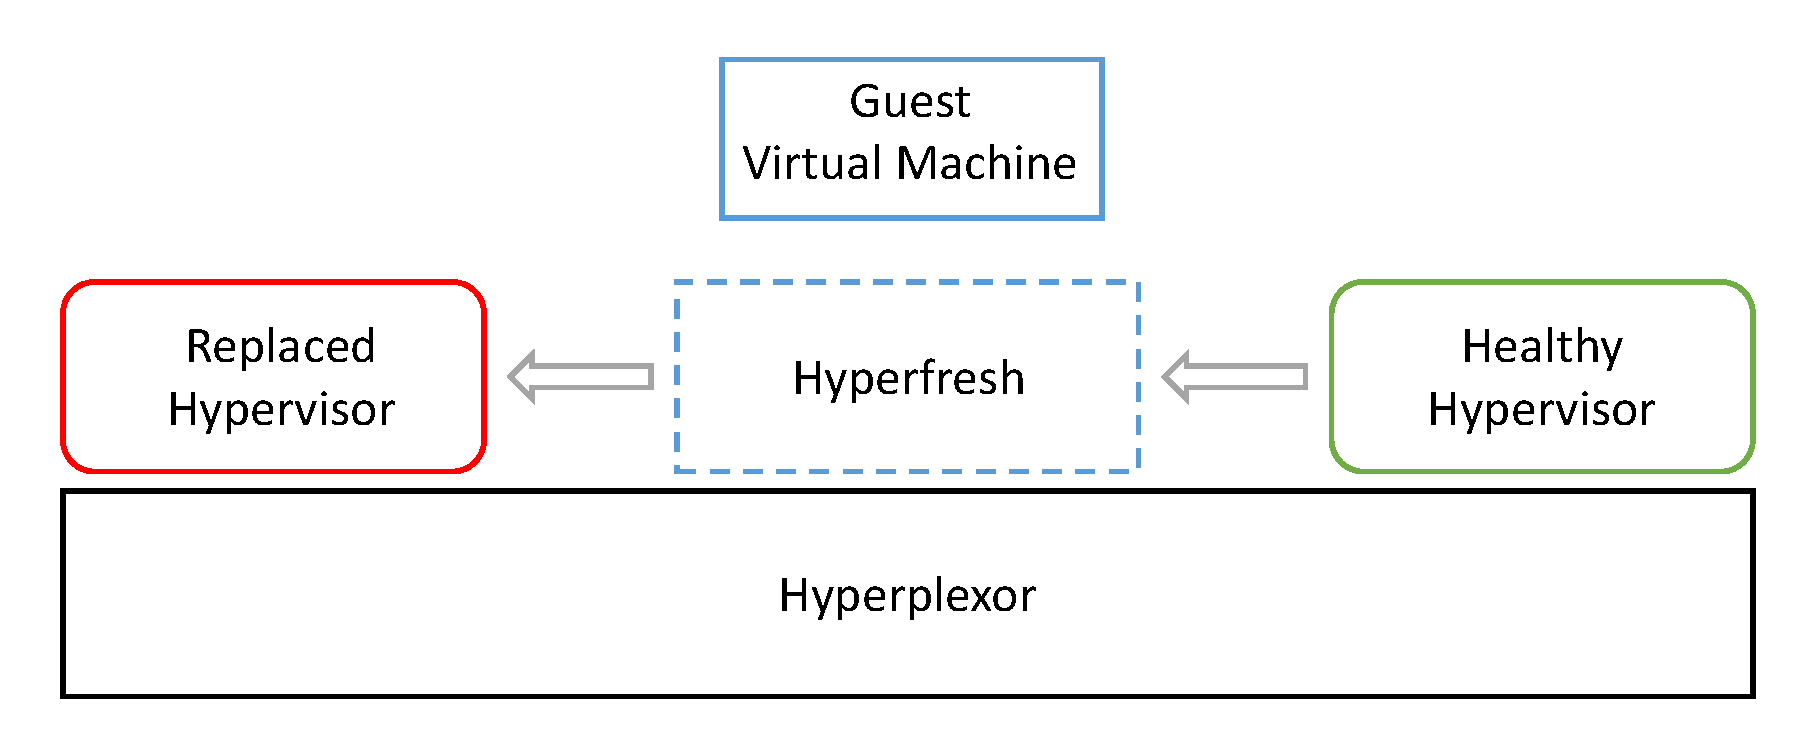
\includegraphics[width=0.5\textwidth]{figures/shift.pdf}
%  \caption{Hypervisor switching operation}
%  \label{fig:switching}
  %\includegraphics[width=15cm,height=6cm,keepaspectratio]{architecture__1_.jpg}
%\end{figure}

%\subsection{Hypervisor Switching}
%The guest initially runs on the hypervisor which in turn runs on thin hyperplexor. The guest pre-allocates it's memory by pinning the pages in memory during boot time. When the current hypervisor requires updates, a new hypervisor with pre-installed updates boots up  and runs the guest in migration state. The guest in migration state maps it's memory in advance to the guest running on current hypervisor using grant table mechanism described above and waits for the VCPU and I/O device state. The guest on current hypervisor is then paused and the VCPU and I/O device state are transferred to the guest on updated hypervisor as shown.

